\documentclass[a4paper, 11pt]{article}
\usepackage{covington}
\usepackage{amssymb}
\usepackage{amsmath}
\usepackage[catalan]{babel}
\usepackage{graphicx}
\usepackage{eurosym}
\usepackage{caption}
\usepackage{subcaption}
\usepackage{float}
\usepackage{bm}
\usepackage{layout}
\usepackage{hyperref}
\textheight=23.94cm 
\textwidth=17cm 
\topmargin=-1cm 
\oddsidemargin=-0.5cm 
 
\newcommand{\header}[4]{
	\begin{center}
		\rule{\linewidth}{0.5pt}
		
		{\small{#1}}
      
        \vspace{0.2in}
        
		{\large{#2}}
		
        \vspace{0.2in}
        
		{\small{#3}}
		
		\vspace{0.15in}
		
		{#4}
		
		\vspace{-0.1in}
		\rule{\linewidth}{0.6pt}
	\end{center}
}

\begin{document}
 
\header{\sc Barcelona Graduate School of Economics \hfill Master's Degree in Data Science}{\bf Statistical Modeling and Inference $-$ Project: Stochastic Gradient Descent}{\sc Group 3: Niti Mishra $\cdot$ Miquel Torrens $\cdot$ B\'alint V\'an}{December 24\textsuperscript{th}, 2015}
% EXERCISE 1
\textbf{\underline{Exercise 1}.} \textit{Find the Fisher Information matrix for logistic regression models.} \\
\newline We take the definition of the Fisher information matrix as:
\begin{eqnarray}
\mathcal{I}(\theta) := -\mathbb{E}[ \nabla \nabla \log p(\mathbf{t} | \mathbf{\theta}, q) ]. \nonumber
\end{eqnarray}
Recall that logit output is Bernouilli distributed (belongs to exponential family) and uses the canonical link as a link function. In such distribution $q=1$. Under the canonical link:
\begin{eqnarray}
\mathcal{I}(\theta) &=& -\mathbb{E}[ \nabla \nabla \log p(\mathbf{t} | \mathbf{\theta}, q) ] \nonumber \\
&=& - \nabla \nabla \log p(\mathbf{t} | \mathbf{\theta}, q). \nonumber
\end{eqnarray}
Thus, in such case the Fisher Information is also the Hessian operator.\\
\newline We recover the exercise on GLM problem set where we generally\footnote{We assume that if the observations are weighted, such weight is normalized so that $\mathbb{E}[\gamma_n] = 1$.} found that with the canonical link:
\begin{eqnarray}
- \nabla \nabla \log p(\mathbf{t} | \mathbf{X}, \mathbf{w}) &=& \sum_{n} q c''(\phi_n^T \mathbf{w}) \phi_n \phi_n^T \nonumber \\
&=& \sum_{n} c''(\phi_n^T \mathbf{w}) \phi_n \phi_n^T. \nonumber
\end{eqnarray}
In the second equation we plug in $q = 1$. The funciton $c''(\phi_n^T \mathbf{w})$ is the variance function, for the logit case its value is $c''(\phi_n^T \mathbf{w}) = p_n (1 - p_n)$, where $p_n$ is the predicted value of our model for observation $n$. Thus:
\begin{eqnarray}
- \nabla \nabla \log p(\mathbf{t} | \mathbf{X}, \mathbf{w}) &=& \sum_{n} p_n (1 - p_n) \phi_n \phi_n^T \nonumber \\
&=& \mathbf{\Phi}^T \mathbf{\Gamma} \mathbf{\Phi}, \nonumber
\end{eqnarray}
where $\mathbf{\Gamma} = \text{diag}\{p_n (1 - p_n)\}$. Hence we conclude:
\begin{eqnarray}
\mathcal{I}(\theta) = \mathbf{\Phi}^T \mathbf{\Gamma} \mathbf{\Phi}. \nonumber
\end{eqnarray}
% EXERCISE 2
\newpage
\textbf{\underline{Exercise 2}.} \textit{Use the first 500K observations from the Higgs data set to calculate the MLE, the Fisher information matrix and, hence obtain the standard errors of the estimators when all features are present.} \\
\newline The MLE parameter estimations are:\\
\newline 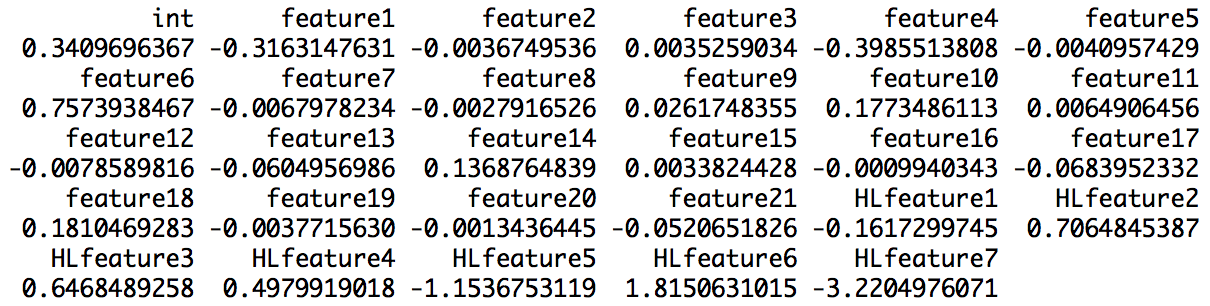
\includegraphics[scale=0.7]{w_mle.png}\\
\newline The first parameter corresponds to the intercept (in R tagged as \texttt{int}).\\
\newline The standard errors of the estimators are calculated by inverting the Hessian matrix and taking the squared root of the resulting diagonal. The outcome is the following:\\
\newline 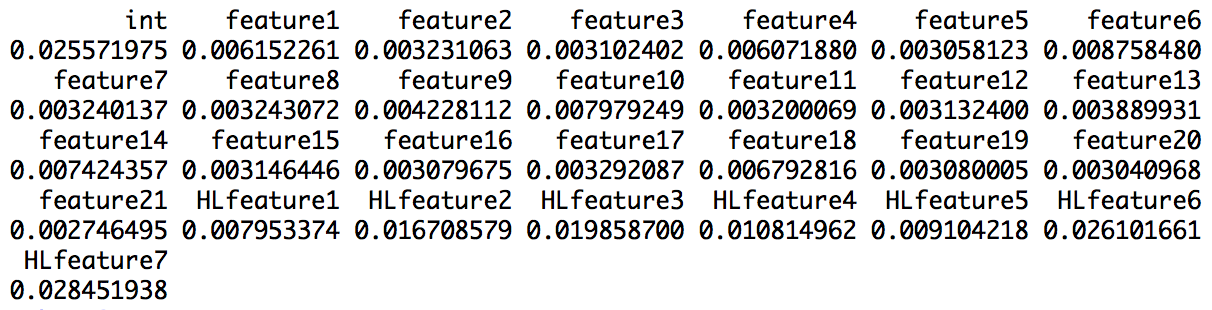
\includegraphics[scale=0.7]{se_wmle.png}\\
\newline For completeness we print the Hessian matrix, in three chunks:\\
\newline 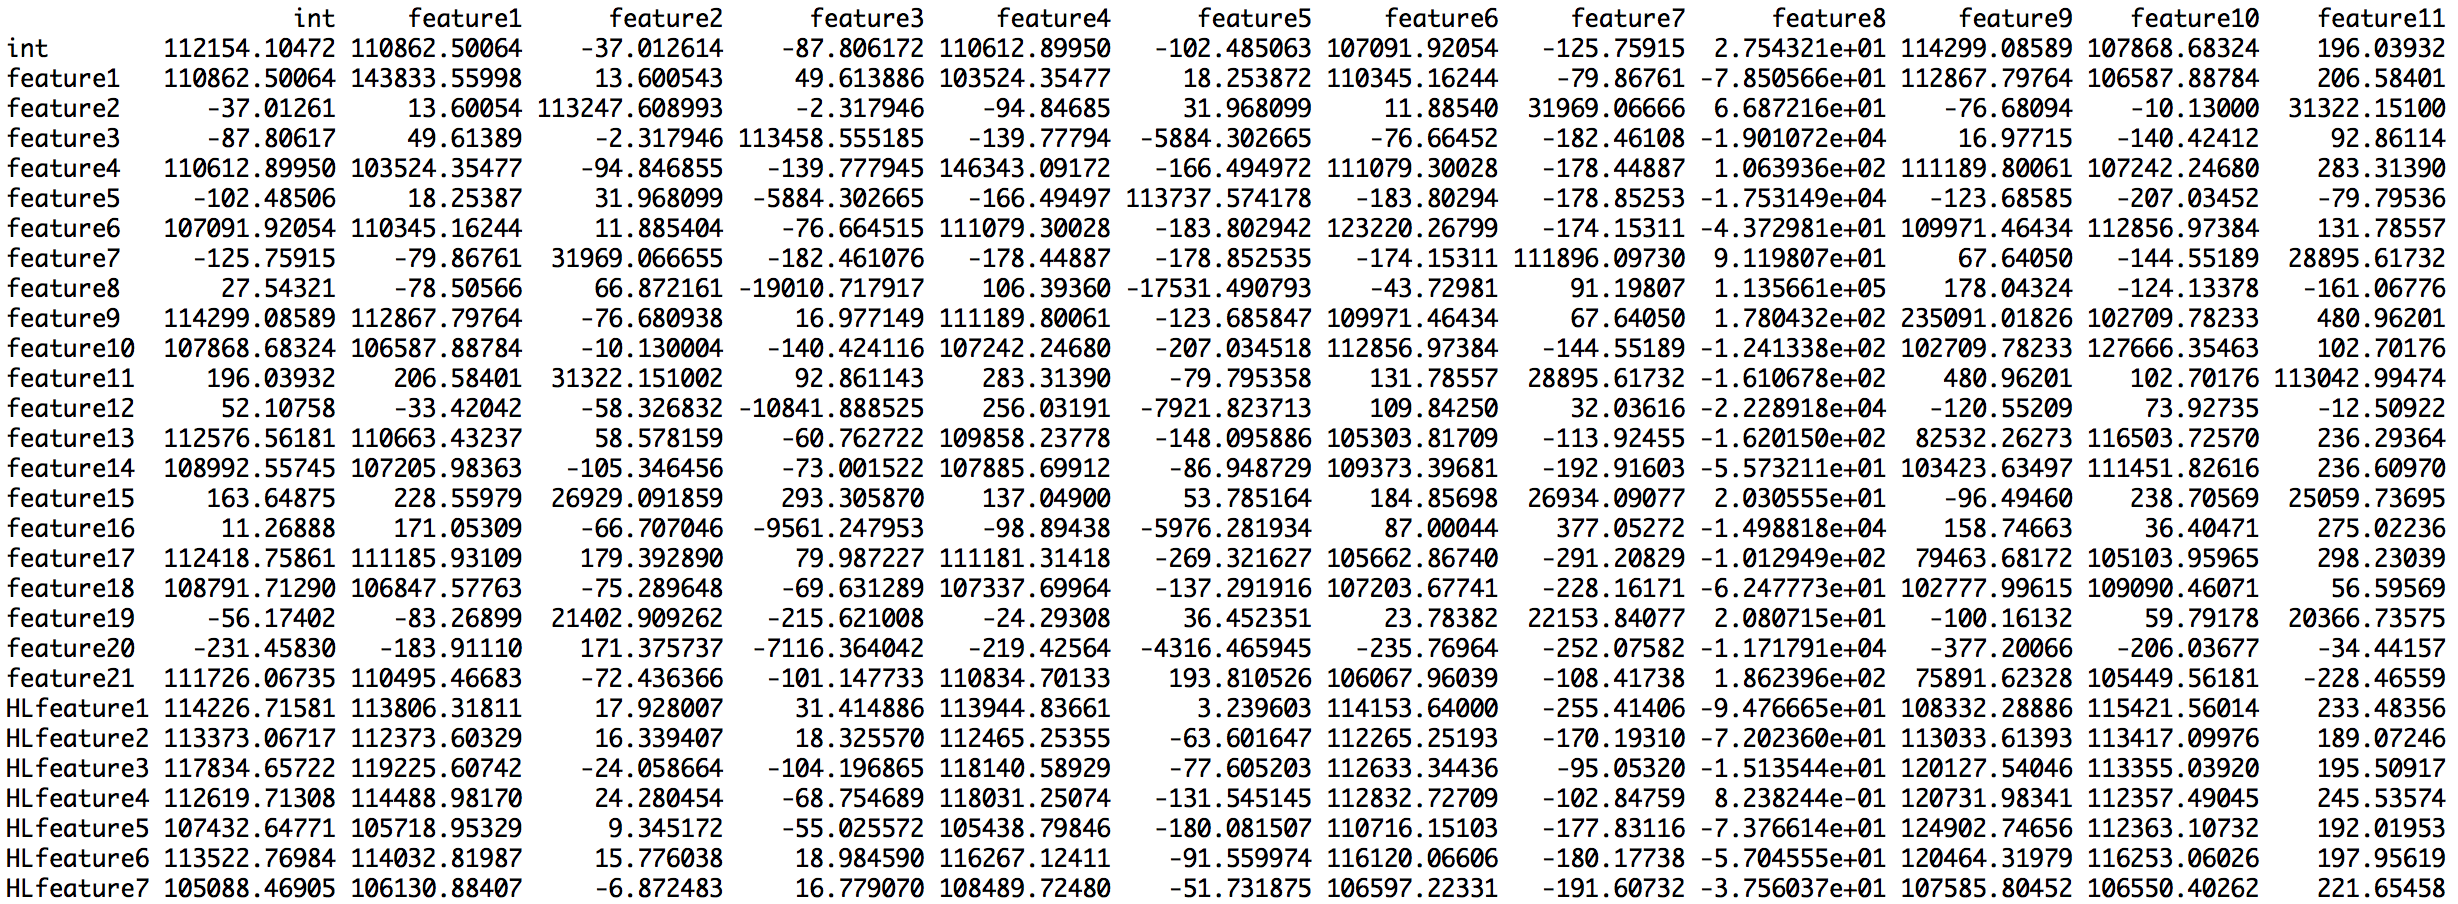
\includegraphics[scale=0.39]{hessian1.png}\\
\newline 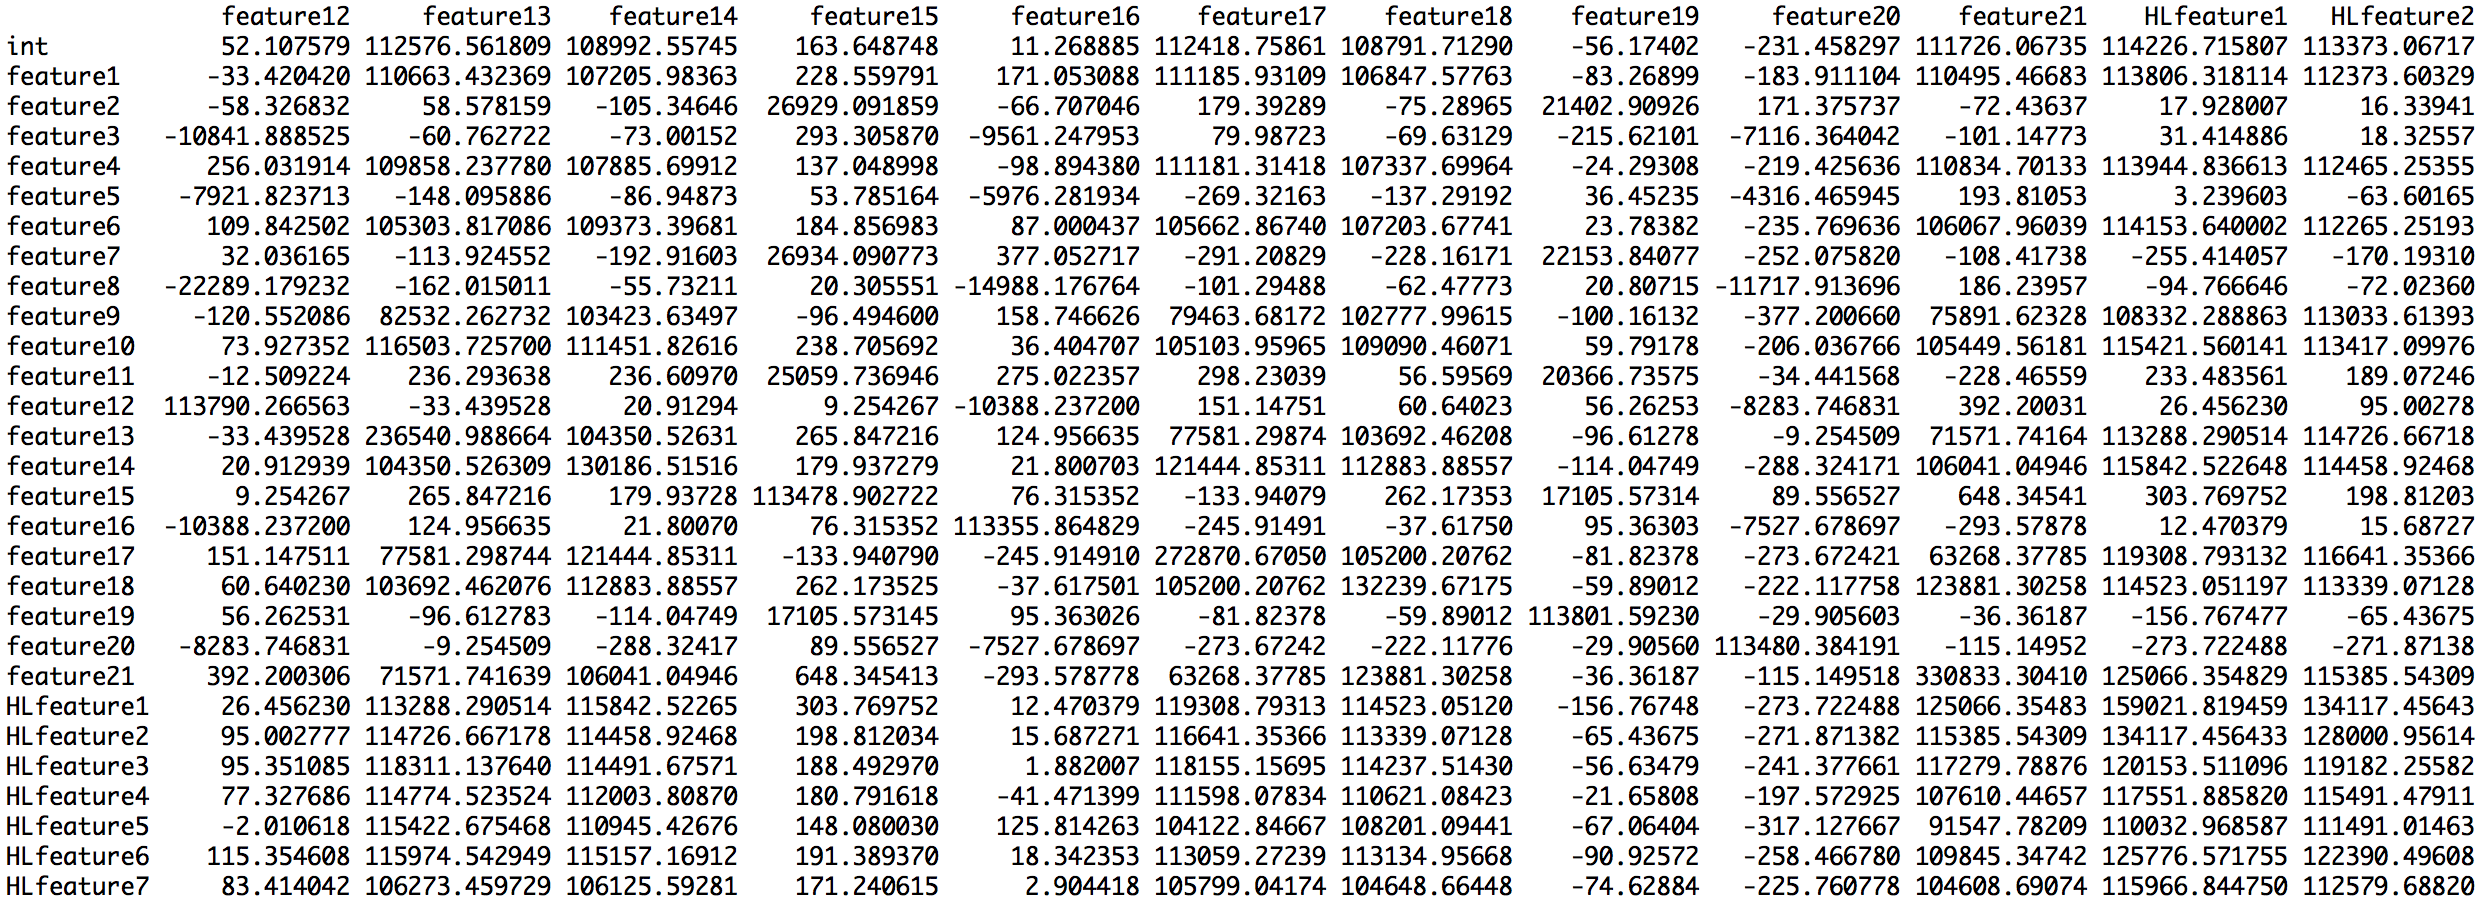
\includegraphics[scale=0.39]{hessian2.png}\\
\newline 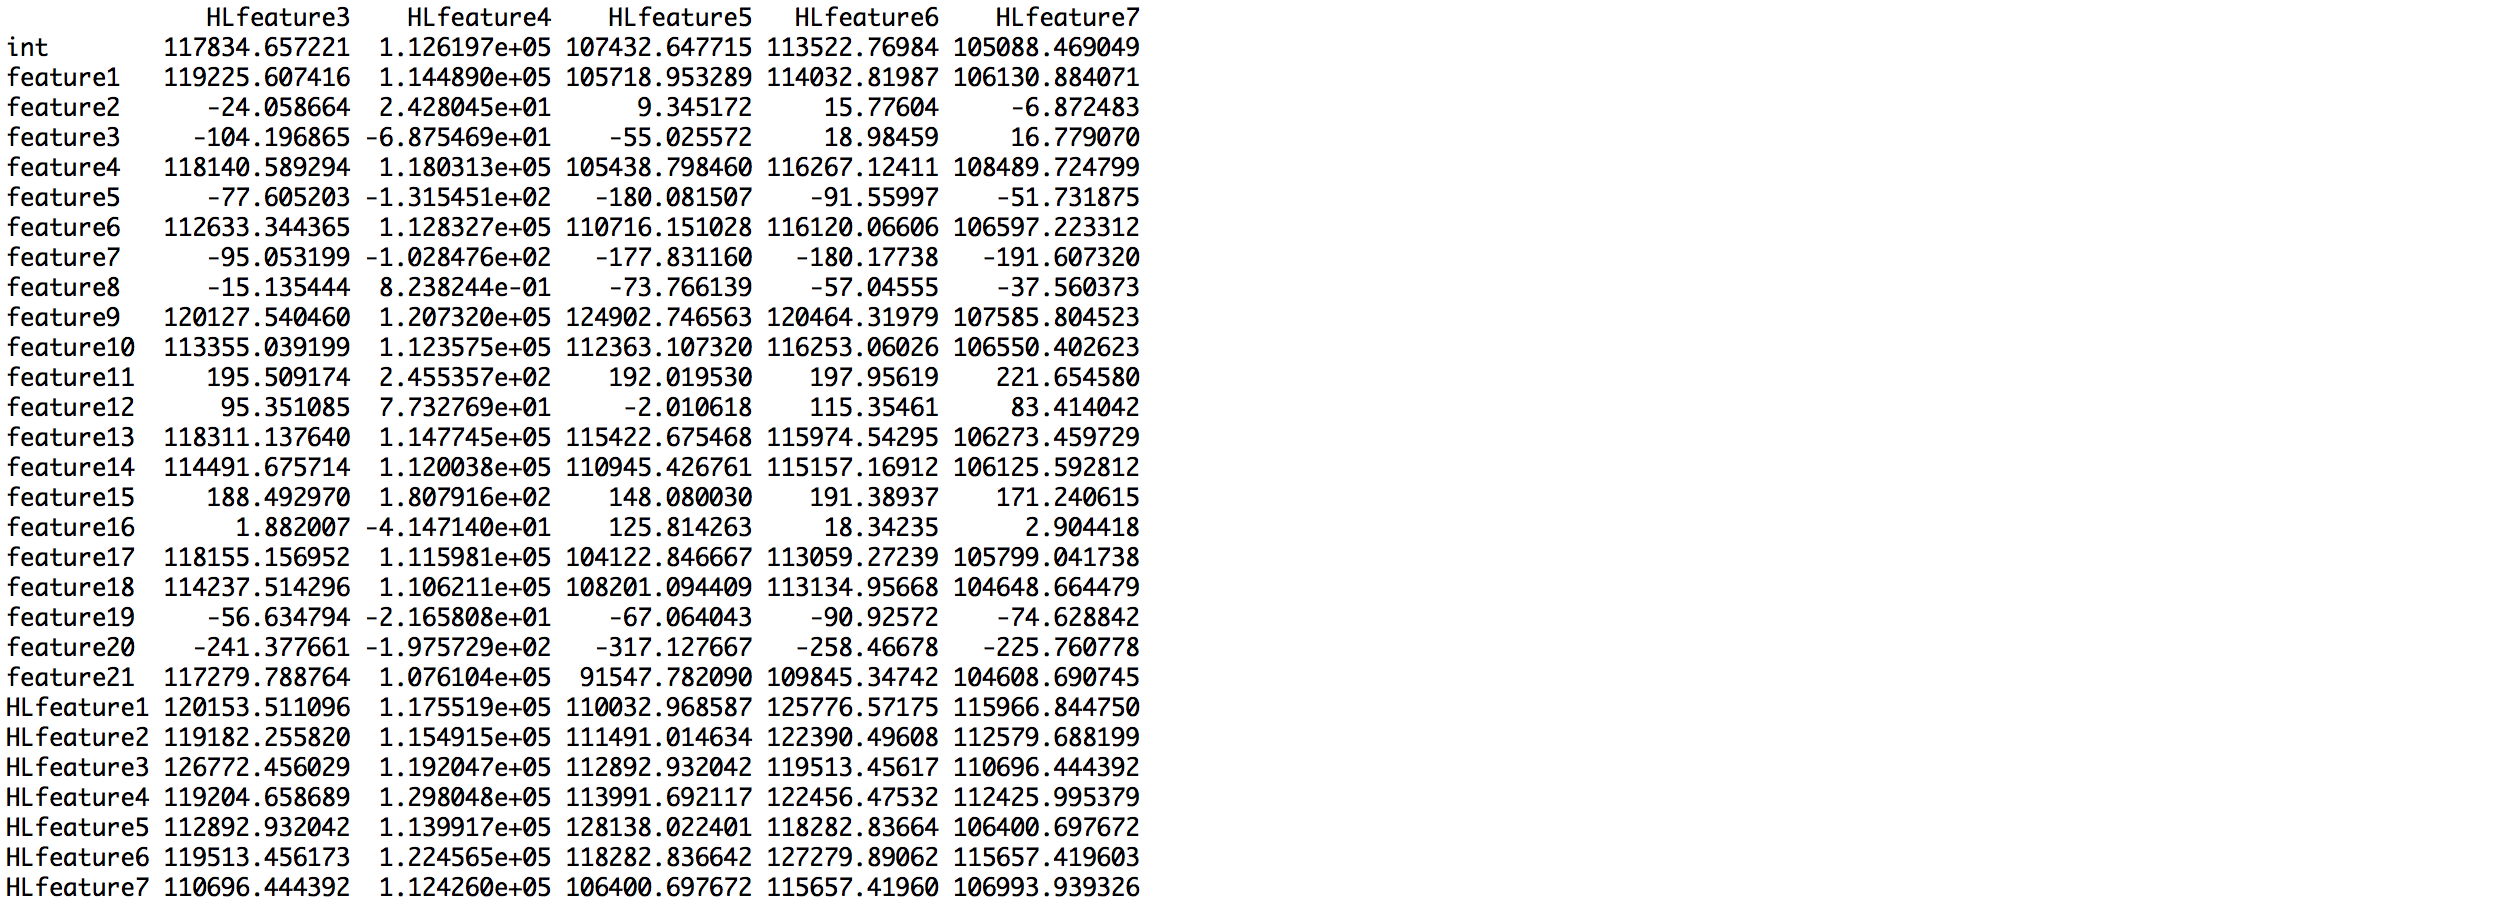
\includegraphics[scale=0.39]{hessian3.png}
% EXERCISE 3
\newpage
\textbf{\underline{Exercise 3}.} \textit{Describe in approximately one page, the methodology of stochastic gradient descent and its default implementation in the sgd R package.}\\
\newline Extremely high time complexity requirement for estimations of big datasets sparked interest in algorithms that utilize only the gradient computations such as Stochastic Gradient Descent ({\sc sgd}). {\sc sgd} is a modification of the Robbins-Monro procedure for recursive estimation that requires linear time complexity in $N$ and sublinear in $p$, which is much better than traditional estimation algorithms such as the Fisher scoring. {\sc sgd} is defined through the following iteration:
\begin{eqnarray}
\theta_{n}^{\text{{\sc sgd}}} = \theta_{n-1}^{\text{{\sc sgd}}} + \gamma_n C_n \nabla \log f(\mathbf{y}_n | \mathbf{x}_n, \theta_{n-1}^{\text{{\sc sgd}}}), \nonumber
\end{eqnarray}
where, the learning rate $\gamma_n$ is defined such that $n \gamma_n \rightarrow \gamma > 0$ as $n \rightarrow \infty$. The sequence $C_n$ is a sequence of positive-definite matrices, such that $C_n \rightarrow C$. It is used to better condition the iteration. This method, known as explicit {\sc sgd}, is efficient, because $\gamma_n$ is just a scalar sequence, $C_n$ is numerically tractable and the log-likelihood is evaluated only in the observation $n$ and not the entire dataset. It is also statistically correct, as it can be shown that it converges to a point where $\mathbb{E}(\nabla \log f(\mathbf{y}_n | \mathbf{x}_n, \theta) = 0$. In exponential familiy models this point is a unique optimum, so it converges to the true parameter value (it is unbiased).\\
\newline We should mention, however, that it is hard to find a learning rate $\gamma$ that converges fast and does not cause numerical divergence, and even for well-behaved values of $\gamma$ convergence and stability are not guaranteed. To solve this, the improvement made is known as the Averaged Implicit Stochastic Gradient Descent ({\sc ai-{\sc sgd}}) method. This is the default implementation of the \texttt{sgd} R package. The {\sc ai-{\sc sgd}} procedure is:
\begin{eqnarray}
\theta_{n}^{\text{im}} = \theta_{n-1}^{\text{im}} + \gamma_n C_n \nabla \log f(\mathbf{y}_n | \mathbf{x}_n, \theta_{n}^{\text{im}}), \nonumber
\end{eqnarray}
with $\bar{\theta}_n = (1/n) \sum_{i=1}^{n} \theta_{i}^{\text{im}}$. Implicit update is the first key component of {\sc ai-{\sc sgd}}. Note that $\theta_{n}^{\text{im}}$ is present on both sides. One can show that this implicit update is a \textit{shrinked} version of the explicit update. This makes it robust to misspecifications of the learning parameter. The second key component is the averaging, which guarantees optimal statistical efficiency under relatively relaxed conditions.\\
\newline A key assumption here is that the direction of the gradient of the likelihood does not depend on the $\theta$. This implies that the implicit update can be performed once a scalar value is found which will scale the gradient appropriately. Hence, the gradient for the implicit iterate $\theta$ is a scaled version of the gradient of the previous iterate.\\
\newline It is also possible to regularize the implicit {\sc sgd} by adding a elastic net penalty to the log-likelihood. Thus, {\sc ai-{\sc sgd}} is effectively a recursive estimation method that is statistically optimal, numerically stable and applicable to big datasets. This analysis leads to an algorithm which implements the most general update of implicit {\sc sgd}.\\
\newline Generally, the algorithm works as follows. To minimize the objective function using {\sc sgd}, we choose initial vector of parameters $\theta$ and the learning rate $\gamma$. The default choice for the parameters in R is $\theta = 0$, and the default learning rate is one-dimensional, of the form:
\begin{eqnarray}
\gamma_n = \gamma_0 (1 + a \gamma_0 n)^{−c}, \nonumber
\end{eqnarray}
where $\gamma_0,a,c \in \mathbb{R}$ are fixed constants set so that they lead to statistical efficiency. Then, we perform the described iterations on independent random permutations of the dataset with a specified number of passes through the data (in R by default, 3) until we obtain an approximate minimum of our objective function. This is proxied by a stopping rule, namely when improvement of the likelihood is small enough (in R this is \texttt{1e-05}). At that point, parameters are stable and the result can be drawn.\\
% EXERCISE 4
\newpage
\textbf{\underline{Exercise 4}.} \textit{Fit the same logistic regression model using stachastic gradient
descent. You should do this for each of 1, 5, 10, ..., 50 passes through the data, starting from the MLE. For each number of passes, repeat the estimation for 50 independent random permutations of the data. As an outcome, you should produce an appropriate figure that illustrates the variability of the estimators due to permutation as a function of the number of passes and compares it to the varibility of MLE.}\\
\newline We produce the following plot:
\begin{center}
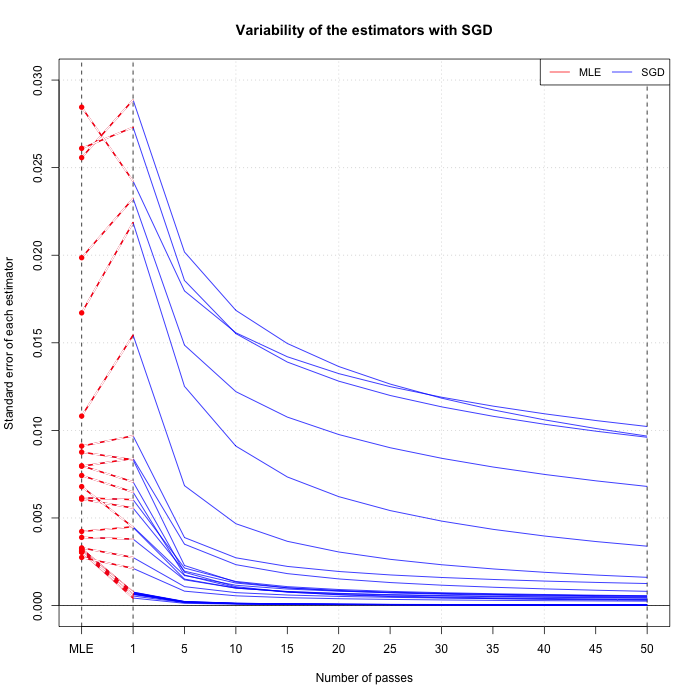
\includegraphics[scale=0.58]{plot_ex4_v3.png}\\
\end{center}
In the first vertical dashed line on the left, we see as red dots the standard error of each of the 29 estimated coefficients under {\sc mle} (anonymized). The red dashed lines point the dots towards their respective standard error using {\sc sgd}. The second vertical dashed line represents these same standard errors evaluated performing {\sc sgd} starting from the {\sc mle}, with 1 pass through the data using 50 independent random permutations of the data. From there we see how this variability evolves as we change the number of passes, up to 50. We observe that with {\sc sgd} more passes through the data help the estandard error of the estimators decrease.\\
\newline To better see these differences, as an extra we also plot the difference in standard errors for {\sc mle} and {\sc sgd}. Positive values mean that those from {\sc mle} are greater, and viceversa. For a small enough number of passes there is no dominant method, but as the number grows {\sc sgd} exhibits smaller variability for all estimators.
\begin{center}
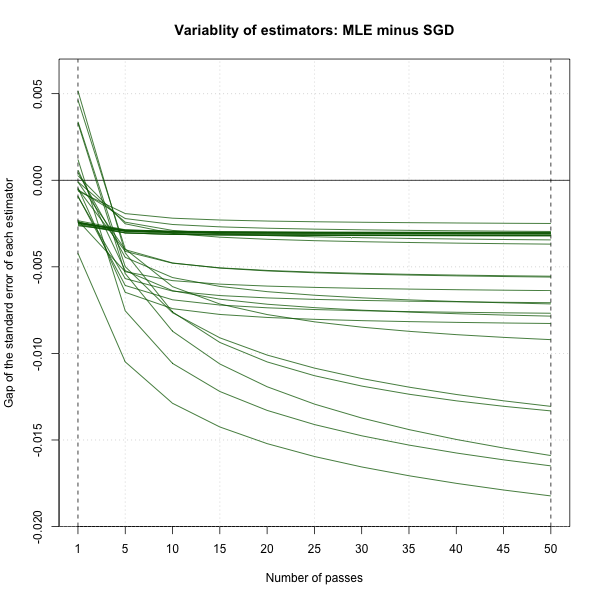
\includegraphics[scale=0.58]{plot_ex4_v2.png}\\
\end{center}

\end{document}
